\chapter{Weak Fields, Gravitational Waves, and the Action Principle}

The lecture opens with exactly the right warning. The full equations of general relativity are unpleasant to work out on a blackboard, and even when one does work them out, the result is not always the most illuminating way to learn the subject. So we will proceed as the lecture proceeds: we will identify the equations, understand what kinds of terms they contain, see why weak disturbances look like waves, separate real geometry from coordinate artifact, and only then turn to the form of the physical solutions. These notes follow Leonard Susskind's lecture closely, with explicit credit to Leonard Susskind, LazyingArt LLC, and Video2Book. Because the sign discussion in this part of the transcript is noisy, we fix one convention once and for all:
\[
\eta_{\mu\nu}=\mathrm{diag}(-1,1,1,1).
\]

\section{Weak Fields and the Vacuum Background}

The lecture begins by saying what kind of problem is under discussion: weak gravitational fields, linearity versus nonlinearity, and gravitational waves. Weakness is not a mood; it is an approximation scheme. If a quantity is small, then higher powers of it are smaller still, and the usual rule is to ignore those higher-order terms. This is why the lecture immediately reformulates the problem as one of perturbations about equilibrium.

So let us first ask what the equilibrium equations are. We take the vacuum theory, with no matter and therefore no energy-momentum tensor on the right-hand side. Einstein's equations are then
\begin{align}
R_{\mu\nu}-\frac12 g_{\mu\nu}R=0.
\end{align}
Taking the trace gives
\begin{align}
g^{\mu\nu}\!\left(R_{\mu\nu}-\frac12 g_{\mu\nu}R\right)=R-2R=0,
\end{align}
and hence
\begin{align}
R=0.
\end{align}
Therefore the vacuum field equations reduce to the simpler form
\begin{align}
R_{\mu\nu}=0.
\end{align}

\begin{figure}[t]
\centering

\includegraphics[width=0.68\textwidth]{lecture_10_figure_02.png}
\caption{The vacuum equation \(R_{\mu\nu}=0\) isolated at the start of the lecture.}
\end{figure}

Now we ask the question posed explicitly in the lecture: what is an equilibrium situation? In the present context it means a solution with no time dependence and no matter on the right-hand side. The lecture insists that there is really only one such background for the discussion at hand: empty flat spacetime, with no curvature and no interesting gravitational field.

But here Susskind inserts a correction that we should keep visible. It is not quite proper to say that the metric \emph{is} \(\eta_{\mu\nu}\). The metric is a tensor, and its components depend on the coordinates. What is true is that in flat spacetime one can choose coordinates in which the metric takes the Minkowski form \(\eta_{\mu\nu}\). That caveat is not a side remark. It is already pointing toward the later problem of fake perturbations created by funny coordinates.

Thus the equilibrium background is not merely ``the matrix \(\eta\).'' It is flat spacetime, together with the statement that there exists an inertial coordinate system in which
\begin{align}
g_{\mu\nu}=\eta_{\mu\nu}.
\end{align}
That is the background about which we now perturb.

\section{Linearizing About Flat Spacetime}

The lecture next turns from the vacuum background to the physical situation we actually care about. Imagine some complicated, violent source far away, a binary pulsar for example. Near the source the field may be strong, and the emitted radiation may be strong as well. But far enough away, the disturbance has spread out. Then the geometry can be chosen to be only slightly different from the flat background.

This is what ``weak'' means in practice. The true metric can be chosen to have the form
\begin{align}
g_{\mu\nu}(x,t)=\eta_{\mu\nu}+h_{\mu\nu}(x,t),
\end{align}
where the components of \(h_{\mu\nu}\) are small compared with those of \(\eta_{\mu\nu}\). The lecture even pauses to note, with characteristic dryness, that the perturbation is called \(h\) simply because \(h\) comes after \(g\).

\begin{figure}[t]
\centering

\includegraphics[width=0.84\textwidth]{lecture_10_figure_03.png}
\caption{The weak-field split on the left and, on the right, the lecture's schematic hierarchy from curvature to Christoffel symbols.}
\end{figure}

What do we do with this? Exactly what the lecture says: we calculate \(R_{\mu\nu}\) from the perturbed metric and set it equal to zero. But instead of writing the full answer, which would be ugly and not very enlightening, the lecture only records the structure of the calculation.

The Christoffel symbols are built from the inverse metric and derivatives of the metric:
\begin{align}
\Gamma^{\rho}{}_{\mu\nu}
=
\frac12\,g^{\rho\sigma}
\bigl(
\partial_{\mu}g_{\sigma\nu}
+
\partial_{\nu}g_{\sigma\mu}
-
\partial_{\sigma}g_{\mu\nu}
\bigr).
\end{align}
On the board this is reduced to the shorthand
\begin{align}
\Gamma \sim \frac12\,g^{-1}\partial g,
\end{align}
and the curvature is likewise summarized as
\begin{align}
R \sim \partial\Gamma+\Gamma\Gamma.
\end{align}
These are not final formulas. They are the lecture's way of exposing the skeleton of the argument.

The next ingredient is the inverse metric. The board writes this only schematically as something like \(\eta-h\). The cleaned first-order statement is
\begin{align}
g^{\mu\nu}=\eta^{\mu\nu}-h^{\mu\nu}+O(h^2),
\end{align}
with indices on \(h\) raised and lowered using \(\eta_{\mu\nu}\) at this order.

\begin{figure}[t]
\centering

\includegraphics[width=0.84\textwidth]{lecture_10_figure_04.png}
\caption{The next board pass sharpens the point that \(\partial\eta=0\), so only derivatives of \(h_{\mu\nu}\) survive at leading order.}
\end{figure}

Now comes the decisive step. In the chosen inertial coordinates,
\begin{align}
\partial_{\alpha}\eta_{\mu\nu}=0,
\end{align}
so the derivative of the full metric is simply
\begin{align}
\partial_{\alpha}g_{\mu\nu}=\partial_{\alpha}h_{\mu\nu}.
\end{align}
Therefore the Christoffel symbols are linear in derivatives of the perturbation,
\begin{align}
\Gamma = O(\partial h),
\end{align}
and the Ricci tensor contains second derivatives of \(h\) together with quadratic corrections:
\begin{align}
R_{\mu\nu}\sim \partial\partial h+(\partial h)(\partial h).
\end{align}
The \(\Gamma\Gamma\) term is quadratic, so in the weak-field approximation it is dropped. Thus the vacuum equations reduce, schematically, to a set of equations built from second derivatives of \(h_{\mu\nu}\). The lecture goes no further than this on the board, and we should not pretend otherwise.

\subsection{Question \& Answer}

A student raises exactly the right objection at this point. The curvature tensor begins with more indices than the Ricci tensor, and contracting indices can reintroduce the metric. Why do those extra factors not spoil the linearized approximation?

The answer is that once the metric is written as \(\eta+h\), every additional factor of \(h\) costs another order of smallness. The Ricci tensor is already made from derivatives of \(h\), so multiplying by one more \(h\) produces something of higher order. Terms of the following kinds are therefore consistently discarded:
\begin{align}
h\,\partial^2 h,
\qquad
h\,\partial h,
\qquad
(\partial h)^2.
\end{align}
This is exactly what the lecture means by linearization: throw away everything of higher power in the small fluctuation. If \(h\sim 10^{-2}\), then quadratic corrections are of order \(10^{-4}\), and that is the logic being used throughout. The approximation is controlled because the neglected terms are of order \(h^2\).

\section{Why Wave Equations Appear}

Once the lecture has reduced the Ricci tensor to second derivatives of the perturbation, it shifts to a simpler and more familiar comparison. Before discussing the solutions in detail, it asks us to recall what an ordinary wave equation looks like.

For a scalar field \(\phi\) moving along the \(z\)-axis, the simplest wave equation is
\begin{align}
\partial_t^2\phi-\partial_z^2\phi=0.
\end{align}
In three spatial dimensions it becomes
\begin{align}
\partial_t^2\phi-\partial_x^2\phi-\partial_y^2\phi-\partial_z^2\phi=0.
\end{align}
The lecture's point is not that gravity is a scalar. The point is that equations built from second time derivatives and second spatial derivatives are exactly the kind of equations that typically describe waves.

Here there is another important spoken beat that is easy to lose in a polished draft. The Einstein equations do not become one scalar wave equation. They become a family of component equations. At first sight \(R_{\mu\nu}=0\) gives sixteen component conditions, although not all are independent. This is why the lecture compares the situation to Maxwell theory: not one equation, but several equations of a similar wave-like form.

Only after the spurious coordinate modes have been removed do the equations settle into the cleaned form one usually writes in notes. In our sign convention that cleaned statement is
\begin{align}
\Box h_{\mu\nu}=0,
\qquad
\Box:=-\partial_t^2+\partial_x^2+\partial_y^2+\partial_z^2.
\end{align}
But the lecture reaches this only in stages. First comes the schematic observation that weak gravity leads to second-derivative equations of wave type. Only later does one sharpen that statement into the familiar linear wave equation for the physical components.

The discussion period adds another clarification that belongs right here. The linearity of the resulting wave equation does \emph{not} come from eliminating fake solutions. It comes from the weak-field approximation itself. General relativity is nonlinear. We have made it linear only by deciding that the square of the perturbation is negligible.

\section{Coordinate Wiggles and Spurious Perturbations}

At this point the lecture interrupts its own forward motion and raises the central conceptual obstacle. Earlier we said that flat space is not the statement \(g_{\mu\nu}=\eta_{\mu\nu}\) in every coordinate system, but rather that one can choose coordinates in which this is true. So if we now write \(g_{\mu\nu}=\eta_{\mu\nu}+h_{\mu\nu}\), how do we know that \(h_{\mu\nu}\) represents real curvature rather than a mere re-coordinatization of flat space?

\subsection{Question \& Answer}

If flat space can already be made to look like \(\eta+h\), what distinguishes a real gravitational perturbation from a coordinate artifact?

The answer is that the appearance of the metric components is not enough. Flat space may acquire a nontrivial-looking metric when we describe it with nontrivial coordinates. The lecture makes this vivid by stepping down from spacetime to the ordinary flat blackboard. The board is flat. Yet we can draw coordinate lines with wiggles. Then the metric components in those coordinates are no longer just the Kronecker delta, even though the geometry has not changed at all.

The lecture writes the coordinate change first in a general form,
\begin{align}
X' = F(x,y),
\qquad
Y' = G(x,y),
\end{align}
and then in the infinitesimal perturbative form actually used in the argument,
\begin{align}
X' &= X+f_x(x,y),\\
Y' &= Y+f_y(x,y).
\end{align}

\begin{figure}[t]
\centering

\includegraphics[width=0.84\textwidth]{lecture_10_figure_05.png}
\caption{The board example of coordinate wiggles: a small deformation of coordinates induces a small correction to the metric on an otherwise flat plane.}
\end{figure}

It is helpful to rewrite the same calculation in clean index notation. Let \(m,n\in\{x,y\}\), and write
\begin{align}
x'^m=x^m+f^m(x).
\end{align}
Then the differentials transform as
\begin{align}
dx'^m=dx^m+\partial_n f^m\,dx^n.
\end{align}
Now begin with the flat Euclidean line element on the blackboard:
\begin{align}
ds^2=\delta_{mn}\,dx'^m dx'^n.
\end{align}
Substituting the transformed differentials and expanding only to first order in \(f\), we find
\begin{align}
\delta_{mn}dx'^m dx'^n
&=
\delta_{mn}
\bigl(dx^m+\partial_p f^m\,dx^p\bigr)
\bigl(dx^n+\partial_q f^n\,dx^q\bigr)\\
&=
\delta_{mn}dx^m dx^n
+
(\partial_m f_n+\partial_n f_m)\,dx^m dx^n
+
O(f^2).
\end{align}
Thus the induced perturbation takes the form
\begin{align}
h_{mn}=\partial_m f_n+\partial_n f_m.
\end{align}
This is a small perturbation of the metric, but it is not a new geometry. It is only a coordinate wiggle.

That is the force of the example. There are solutions of the linearized equations that look nontrivial but represent nothing more than flat spacetime in curvilinear coordinates. To get the physical waves, one must impose further conditions that remove these spurious modes. The lecture does not dwell on the detailed gauge equations here; it only stresses their purpose.

\begin{figure}[t]
\centering
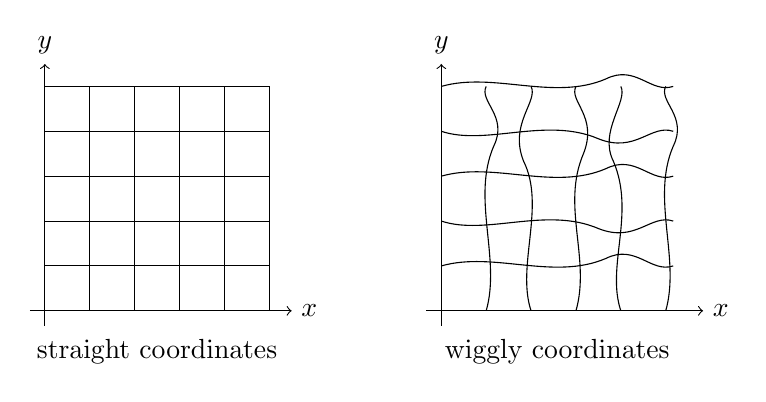
\begin{tikzpicture}[scale=0.95]
\begin{scope}
\draw[->] (-0.2,0) -- (3.3,0) node[right] {$x$};
\draw[->] (0,-0.2) -- (0,3.3) node[above] {$y$};
\foreach \u in {0.6,1.2,1.8,2.4,3.0}
{
\draw (\u,0) -- (\u,3.0);
\draw (0,\u) -- (3.0,\u);
}
\node at (1.5,-0.55) {straight coordinates};
\end{scope}
\begin{scope}[xshift=5.3cm]
\draw[->] (-0.2,0) -- (3.5,0) node[right] {$x$};
\draw[->] (0,-0.2) -- (0,3.3) node[above] {$y$};
\draw (0.6,0) .. controls (0.8,0.7) and (0.4,1.5) .. (0.7,2.2) .. controls (0.9,2.6) and (0.5,2.8) .. (0.6,3.0);
\draw (1.2,0) .. controls (1.0,0.6) and (1.4,1.4) .. (1.1,2.0) .. controls (0.9,2.5) and (1.3,2.8) .. (1.2,3.0);
\draw (1.8,0) .. controls (2.0,0.7) and (1.6,1.4) .. (1.9,2.1) .. controls (2.1,2.6) and (1.7,2.8) .. (1.8,3.0);
\draw (2.4,0) .. controls (2.2,0.6) and (2.6,1.3) .. (2.3,2.0) .. controls (2.1,2.4) and (2.5,2.8) .. (2.4,3.0);
\draw (3.0,0) .. controls (3.2,0.7) and (2.8,1.5) .. (3.1,2.2) .. controls (3.3,2.6) and (2.9,2.8) .. (3.0,3.0);
\draw (0,0.6) .. controls (0.7,0.8) and (1.5,0.4) .. (2.2,0.7) .. controls (2.6,0.9) and (2.8,0.5) .. (3.1,0.6);
\draw (0,1.2) .. controls (0.6,1.0) and (1.4,1.4) .. (2.1,1.1) .. controls (2.6,0.9) and (2.8,1.3) .. (3.1,1.2);
\draw (0,1.8) .. controls (0.7,2.0) and (1.5,1.6) .. (2.2,1.9) .. controls (2.6,2.1) and (2.8,1.7) .. (3.1,1.8);
\draw (0,2.4) .. controls (0.6,2.2) and (1.4,2.6) .. (2.1,2.3) .. controls (2.6,2.1) and (2.8,2.5) .. (3.1,2.4);
\draw (0,3.0) .. controls (0.7,3.2) and (1.5,2.8) .. (2.2,3.1) .. controls (2.6,3.3) and (2.8,2.9) .. (3.1,3.0);
\node at (1.55,-0.55) {wiggly coordinates};
\end{scope}
\end{tikzpicture}
\caption{A clean redraw of the lecture's point: the plane remains flat while the coordinate lines themselves acquire small ripples.}
\end{figure}

\section{Transverse-Traceless Waves and the Two Polarizations}

Only after this obstacle has been faced does the lecture turn to the physical wave itself. Once the fake coordinate solutions are removed, the remaining equations simplify dramatically: the components of the perturbation satisfy ordinary wave equations, together with further constraints. The lecture then makes the analogy to electromagnetism explicit. Just as electromagnetic waves are transverse, gravitational waves are transverse too.

So let us suppose the wave is moving down the \(z\)-axis. Then the physical components with time indices vanish, and the components parallel to the direction of motion vanish as well:
\begin{align}
h_{0\mu}=0,
\qquad
h_{z\mu}=0.
\end{align}
The only nonzero physical components lie in the plane perpendicular to the direction of propagation. If \(i,j\in\{x,y\}\), the wave takes the form
\begin{align}
h_{ij}(t,z)=h_{ij}^{0}\sin k(z-t),
\end{align}
with
\begin{align}
h_{xy}=h_{yx}.
\end{align}
The trace condition coming from Einstein's equations is
\begin{align}
h_{xx}+h_{yy}=0.
\end{align}
Thus the transverse perturbation is traceless. At each fixed \(z\) and \(t\), the metric in the transverse plane is just a \(2\times2\) symmetric traceless matrix.

\begin{figure}[t]
\centering

\includegraphics[width=0.84\textwidth]{lecture_10_figure_06.png}
\caption{Board evidence for the transverse wave moving along the \(z\)-axis, together with the traceless condition \(h_{xx}+h_{yy}=0\).}
\end{figure}

Since the amplitude notation in the frame is partially blurred, it is better to rewrite the result in a clean basis. A general transverse-traceless wave propagating along \(z\) may be written as
\begin{align}
h_{ij}(t,z)
=
\left[
\begin{pmatrix}
h_{+} & 0\\
0 & -h_{+}
\end{pmatrix}
+
\begin{pmatrix}
0 & h_{\times}\\
h_{\times} & 0
\end{pmatrix}
\right]
\sin k(z-t).
\end{align}
Equivalently, the two independent polarization tensors are
\begin{align}
h^{(+)}_{ij}
=
\begin{pmatrix}
h_{+} & 0\\
0 & -h_{+}
\end{pmatrix},
\qquad
h^{(\times)}_{ij}
=
\begin{pmatrix}
0 & h_{\times}\\
h_{\times} & 0
\end{pmatrix}.
\end{align}
That is all there is. Every physical wave moving along the \(z\)-axis is a linear superposition of these two transverse patterns. The phase \(k(z-t)\) tells us at once that the wave travels with the speed of light.

\begin{figure}[t]
\centering
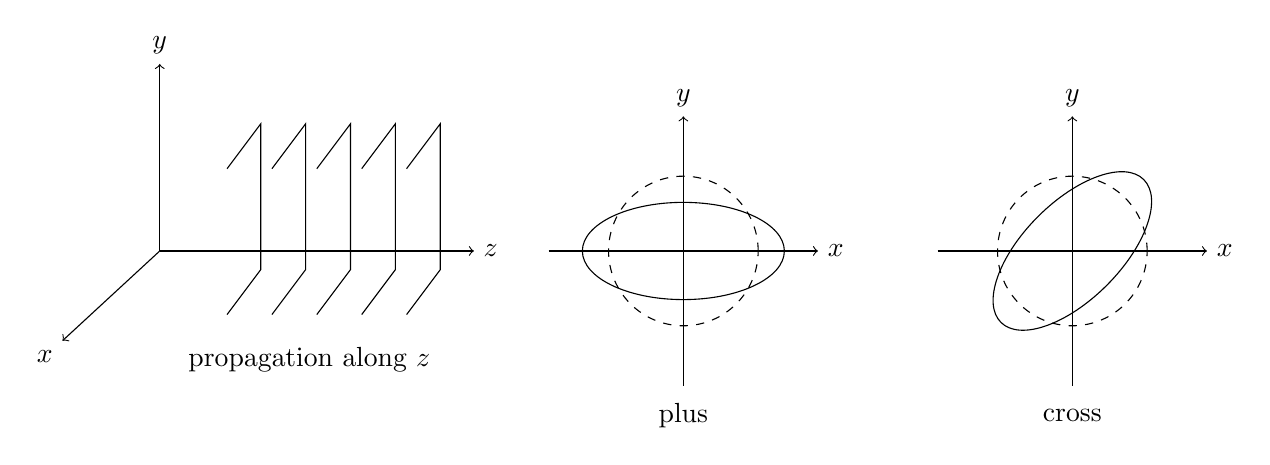
\begin{tikzpicture}[scale=0.95]
\begin{scope}
\draw[->] (0,0) -- (4.2,0) node[right] {$z$};
\draw[->] (0,0) -- (0,2.5) node[above] {$y$};
\draw[->] (0,0) -- (-1.3,-1.2) node[below left] {$x$};
\foreach \s in {0.9,1.5,2.1,2.7,3.3}
{
\draw (\s,1.1) -- (\s+0.45,1.7) -- (\s+0.45,-0.25) -- (\s,-0.85);
}
\node at (2.0,-1.45) {propagation along \(z\)};
\end{scope}
\begin{scope}[xshift=7.0cm]
\draw[->] (-1.8,0) -- (1.8,0) node[right] {$x$};
\draw[->] (0,-1.8) -- (0,1.8) node[above] {$y$};
\draw[dashed] (0,0) circle (1.0);
\draw (0,0) ellipse (1.35 and 0.65);
\node at (0,-2.2) {plus};
\end{scope}
\begin{scope}[xshift=12.2cm]
\draw[->] (-1.8,0) -- (1.8,0) node[right] {$x$};
\draw[->] (0,-1.8) -- (0,1.8) node[above] {$y$};
\draw[dashed] (0,0) circle (1.0);
\draw[rotate=45] (0,0) ellipse (1.35 and 0.65);
\node at (0,-2.2) {cross};
\end{scope}
\end{tikzpicture}
\caption{A clean redraw of the lecture's geometry: propagation along \(z\), together with the plus and cross deformations of the transverse plane.}
\end{figure}

\section{What the Wave Does to Matter}

Now comes the most vivid part of the lecture: what does this actually mean geometrically? Susskind asks exactly the right question. What does it mean to have an \(h_{xx}\)?

Fix \(z\) and \(t\), and look at the transverse plane. The induced metric there is
\begin{align}
ds_{\perp}^{2}
=
(1+h_{xx})\,dx^{2}
+
2h_{xy}\,dx\,dy
+
(1+h_{yy})\,dy^{2}.
\end{align}
For a pure plus mode \(h_{xy}=0\) and \(h_{yy}=-h_{xx}\), so
\begin{align}
g_{xx}=1+h_{xx},
\qquad
g_{yy}=1-h_{xx}.
\end{align}
If \(h_{xx}>0\), then proper distances along the \(x\)-direction are a little larger than they would be in flat space, while those along the \(y\)-direction are a little smaller. Half a cycle later the sine changes sign, and the effect reverses. The lecture wants us to picture precisely this: a square object alternately stretched horizontally and squeezed vertically, then squeezed horizontally and stretched vertically.

For the cross mode the same phenomenon occurs after a rotation by \(45^\circ\). There is no third kind of wave hiding here. The cross mode is the same basic squeeze-and-stretch pattern seen in a rotated basis.

There is, however, one subtlety the lecture insists on. If we had a static deformation, with no oscillation, much of what we were describing would be indistinguishable from a mere redefinition of coordinates. What makes the wave physically unmistakable is that it oscillates. The changing sign of the perturbation produces alternating tidal effects.

\subsection{Question \& Answer}

Is the meter stick itself changing, or should we think instead of two free test masses?

The lecture's answer is deliberately practical. A real meter stick is held together by internal forces. A steel rod and a wooden rod will not respond identically to the same passing wave. So one should not imagine a perfectly rigid standard ruler moving through the wave untouched. The wave carries real curvature, and that curvature creates real stresses and strains in matter. A strain gauge can register those stresses. Two separated test masses can register the induced relative motion even more cleanly.

In this sense the lecture moves from coordinates to mechanics. The wave is not simply making labels on space expand and contract. It is exerting tidal forces. A square piece of plywood is not merely relabeled; it is alternately deformed one way and then the other.

\subsection{Question \& Answer}

If \(h_{0\mu}=0\), does that mean there is no curvature in the time direction?

No. The vanishing of the time-index components is a statement about the allowed physical components of the perturbation in the transverse-traceless description. Curvature is built from derivatives of the surviving \(h_{ij}\), and those components depend on time as well as position. In particular,
\begin{align}
\partial_t h_{ij}\neq 0,
\qquad
R_{\mu\nu\rho\sigma}\sim \partial\partial h.
\end{align}
So even though the perturbation itself lives in the transverse spatial plane, its time dependence enters the curvature tensor. The lecture compares this to electromagnetism: a wave moving along \(z\) may be described entirely by transverse components and yet still be fully dynamical in time.

\section{Sources, Detection, and Another Way of Thinking}

At this stage the lecture broadens the picture again. We have classified the physical weak waves. Now we ask where they come from, how one might detect them, and how the whole theory can be recast in the language of action principles.

\subsection{Sources and Detection}

Accelerating masses generate gravitational waves in much the same way that accelerating charges generate electromagnetic radiation. The lecture's standard example is the binary pulsar: two compact masses orbiting one another in a strong gravitational field. Near the source, the field is too strong for the weak approximation to be trustworthy. Farther away, the radiation spreads out, the metric perturbation becomes small, and the linearized theory becomes a good approximation.

That far-zone weakness matters because the actual strains are tiny. The lecture quotes the astonishing scale \(10^{-21}\) for the dimensionless strain expected from distant sources. That is why detection requires either resonance or interferometric sensitivity. A detector must provide a system that the wave can drive. This is the point of the lecture's discussion of strain gauges, suspended masses, and interferometers: the wave produces a differential transverse effect, and the apparatus must be able to respond to that effect.

The lecture also stresses the speed of propagation. The phase \(z-t\) tells us directly that the wave travels at the speed of light. So too does the broader analogy with electromagnetism. Gravitational waves and electromagnetic waves are, in the lecture's language, the stiffest possible waves.

Then comes the historical evidence. Long before direct detection, there was indirect evidence from the binary pulsar. Radiation carries energy away. If a binary system emits gravitational radiation, its orbital motion must drift correspondingly. The lecture emphasizes that the observed timing of the binary pulsar changes by exactly the amount expected if the system is radiating gravitationally. This is the lecture's payoff: the waves are not just formal solutions. They are real enough to drain energy from an astrophysical system in precisely the predicted way.

The wave discussion closes with two final reminders from the question period. First, the linear approximation is good only when \(h\) is small; the omitted corrections are of order \(h^2\). Second, if the waves are no longer weak, then the nonlinearity of general relativity reappears. Strong gravitational waves do not simply pass through one another without interaction; they scatter. What survives from the weak discussion is the basic transverse character, not the full linear superposition principle.

\subsection{Another Way of Thinking: The Action Principle}

With a little time left, the lecture changes register and announces ``another way of thinking'' about Einstein's equations. Instead of working directly with the field equations, we ask for an action whose stationary points reproduce them.

The lecture frames this in the general language of field theory. A field history is an assignment of field values at every point of spacetime. Not every conceivable field history is a solution. The physical histories are the ones that make the action stationary, once suitable boundary data have been fixed.

Before writing the gravitational action, the lecture first reconstructs the invariant volume element. In two spatial dimensions, suppose the metric is diagonal:
\begin{align}
ds^{2}=g_{xx}\,dx^{2}+g_{yy}\,dy^{2}.
\end{align}
Then the proper side lengths of a small rectangle are \(\sqrt{g_{xx}}\,dx\) and \(\sqrt{g_{yy}}\,dy\), so its area is
\begin{align}
dA=\sqrt{g_{xx}}\,dx\,\sqrt{g_{yy}}\,dy.
\end{align}
Once off-diagonal terms are included, the product \(g_{xx}g_{yy}\) is replaced by the determinant. Thus the general answer is
\begin{align}
dA=\sqrt{\det g}\,dx\,dy.
\end{align}
In three dimensions this becomes
\begin{align}
dV=\sqrt{\det g}\,dx\,dy\,dz.
\end{align}
And in spacetime we pass to the invariant four-volume element
\begin{align}
dV_{4}=\sqrt{|g|}\,d^{4}x,
\end{align}
where \(g=\det(g_{\mu\nu})\).

Now comes the central invariant construction. If \(S(x)\) is any scalar, then
\begin{align}
\int d^{4}x\,\sqrt{|g|}\,S(x)
\end{align}
is invariant under coordinate changes. This is exactly the kind of object an action in general relativity should be, since the laws of physics ought not depend on the coordinates used to write them down.

For pure gravity in vacuum, the natural scalar built from the metric is the scalar curvature \(R\). This leads to the Einstein-Hilbert action
\begin{align}
S_{\mathrm{grav}}=\int d^{4}x\,\sqrt{|g|}\,R.
\end{align}
The lecture then points out that one may also add a constant scalar term, the cosmological constant:
\begin{align}
S_{\Lambda}=\Lambda\int d^{4}x\,\sqrt{|g|}.
\end{align}
This term is just proportional to spacetime volume itself. The lecture is careful not to mix it into the earlier wave discussion; the weak-field equations we have been using are the vacuum equations without the cosmological constant.

Matter enters by the same general logic. One adds further invariant scalar densities built from the relevant fields. In the electromagnetic case, for example, the lecture points to the field tensor \(F_{\mu\nu}\): from it one builds the electromagnetic contribution to the action, again multiplied by the invariant measure \(\sqrt{|g|}\,d^{4}x\).

The conceptual content is clean even if the actual variation is long. One varies the metric, makes the action stationary, and recovers Einstein's equations. The lecture dwells on the contrast: the computation is tedious, but the principle behind it is remarkably simple. It is also part of the lecture's tone that this final calculation is not performed in detail. The action principle is offered as a conceptual coda, not as a second blackboard marathon.

\section{Summary}

The lecture unfolds in a very deliberate order. First, weak fields are defined as small perturbations about an equilibrium vacuum background. Then the metric is written as \(g_{\mu\nu}=\eta_{\mu\nu}+h_{\mu\nu}\), and the field equations are reduced schematically to second derivatives of \(h_{\mu\nu}\). This already tells us that weak gravitational disturbances should behave like waves. But before we are allowed to trust that conclusion, the lecture interrupts itself with the crucial warning that flat space can also look like \(\eta+h\) in wiggly coordinates. Only after those spurious perturbations are removed do the physical transverse-traceless waves emerge, with their two polarization patterns and their real tidal effects on matter. The chapter then closes where the lecture closes: with the broader statement that the same vacuum Einstein equations may be viewed as the stationarity condition of the Einstein-Hilbert action, built from invariant spacetime volume and scalar curvature.